% This template was inspired by public templates from  Prof. Naumann's chair (https://hpi.de/naumann/teaching/master-theses.html) and Prof. Polze's chair (https://www.dcl.hpi.uni-potsdam.de/media/theses/)
\documentclass[
        a4paper,     
%        titlepage,   
        twoside,     
        parskip,     % no indent after paragraph
        % per default headings are set in another font
        % see https://tex.stackexchange.com/questions/289853/why-does-koma-script-mix-serifs-and-sans-serifs/289867#289867
        headings=standardclasses,
        headings=big,
        chapterprefix=false
        ]{scrreprt}

% ======== PACKAGES ========
% language and font encodings
\usepackage[T1]{fontenc}
\usepackage[utf8]{inputenc}
\usepackage[ngerman,english]{babel}

\usepackage[square]{natbib}
\setcitestyle{numbers}

\usepackage[plain]{fancyref} % plain omits stuff like "fig 1 on the following page", use vario if you want that
\usepackage[colorlinks=false]{hyperref}
\usepackage{url}
\usepackage{abstract}  % control abstract (e.g. title)
\usepackage{textcomp}
\usepackage{amsmath}
\usepackage{amssymb}
\usepackage{multirow}
\usepackage{tabularx}
\usepackage{tabulary}
\usepackage{caption}
\usepackage{graphicx}
\usepackage{subcaption}

\usepackage{lipsum}
\usepackage{todonotes}
\usepackage{qtree} % trees https://en.wikibooks.org/wiki/LaTeX/Linguistics
\usepackage[noabbrev]{cleveref} % \cref{eq2,eq1}

\usepackage{fourier} 
\usepackage{array}
\usepackage{makecell}
\usepackage{listings}
\usepackage{tikz}
\usepackage{attrib}
\usepackage[export]{adjustbox} % https://tex.stackexchange.com/questions/296624/subfloat-vertical-alignment-in-latex
\usepackage{xparse}
\usepackage[shortlabels]{enumitem}
\setlist[description]{%
  font={\normalfont\bfseries}
}
\usepackage{placeins} % \FloatBarrier
\usepackage{soul} % \st - strikethough

\usepackage{pdfpages} % includepdf for KOMA titlepage


\renewcommand{\arraystretch}{1.5} % table row spacing

\interfootnotelinepenalty=10000

\NewDocumentCommand{\footurl}{o m}
{\footnote{\IfValueT{#1}{#1~--~}\url{#2} \mbox{(last accessed \today)}}}

\newcommand{\sref}[1]{(\subref{#1})}



% ======== DEFINITIONS ========
\newcommand{\R}{\mathbb{R}}

%https://tex.stackexchange.com/questions/2441/how-to-add-a-forced-line-break-inside-a-table-cell
\renewcommand\theadalign{cb}
\renewcommand\theadfont{\bfseries}
\renewcommand\theadgape{\Gape[4pt]}
\renewcommand\cellgape{\Gape[4pt]}

\pagestyle{headings}

\begin{document}

\includepdf{titlepage}
\cleardoublepage

% ======== DECLARATION ========
\renewcaptionname{english}{\abstractname}{Eidesstattliche Erklärung}
\begin{abstract}
Hiermit versichere ich an Eides statt, dass ich die vorliegende Masterarbeit ohne fremde Hilfe angefertigt und keine anderen als die angegebenen Quellen und Hilfsmittel benutzt habe. Alle Teile, die wörtlich oder sinngemä{\ss} einer Veröffentlichung entstammen, sind als solche kenntlich gemacht. Die Arbeit wurde noch nicht veröffentlich oder einer anderen Prüfungsbehörde vorgelegt. 

Ort, Datum, Name: \hrulefill

\hspace*{0mm}\phantom{Ort, Datum, Name: }Johannes Jasper
\end{abstract}
\clearpage

% ======== ABSTRACT ========
\renewcaptionname{english}{\abstractname}{Abstract}
\begin{abstract} % english abstract
\lipsum[1-3]
\end{abstract}
%---------
\clearpage
\begin{otherlanguage}{ngerman}  % german abstract
\begin{abstract}
\lipsum[1-3]
\end{abstract}
\end{otherlanguage}

\clearpage

% ======== ACKNOWLEDGEMENTS ========
\renewcaptionname{english}{\abstractname}{Acknowledgements}
\begin{abstract}
\lipsum[1-2]    

Thank you.

\end{abstract}

%\clearpage
\cleardoublepage
% ======== TOC ========
\pagenumbering{gobble} % ensures the TOC has no page numbers
\tableofcontents
\clearpage


% ======== CONTENT ========
\pagenumbering{arabic} % re-enables page numbering
\setcounter{page}{1} % resets the page counter

\chapter{Sample Chapter}\label{chap:sample}

Some text with a reference to \fref{sec:sample}.

\section{Sample section}\label{sec:sample}

\begin{figure}[ht]
    \centering
    \begin{subfigure}[b]{0.45\textwidth}
        \centering
        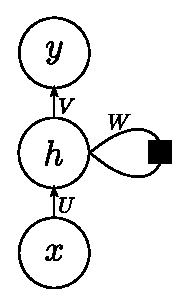
\includegraphics[height=3.2cm]{img/rnn}
        \caption{Description}
        \label{fig:a}
    \end{subfigure}
    ~
    \begin{subfigure}[b]{0.45\textwidth}
        \centering
        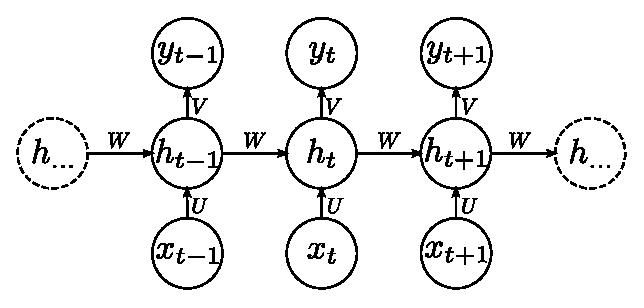
\includegraphics[height=3.2cm]{img/rnn_unfolded}
        \caption{Description}
        \label{fig:b}
    \end{subfigure}
    \caption{Long Description of \fref{fig:a} and \fref{fig:b}. Adapted from~\cite{Goodfellow-et-al-2016}}
    \label{fig:rnns}
\end{figure}

This subsection includes a float containing two figures, as shown in \fref{fig:rnns}. Also, I would like to show off the use of footurls\footurl[It can take additional text]{https://example.com}, which automatically format the URL and add a time stamp.



% ======== BIBLIOGRAPHY ========
\clearpage
\bibliographystyle{plainnat}
\bibliography{bibliography/library}

\end{document}
